\section{HTTPS interception}

\begin{frame}{Attaque HTTPS interception}
    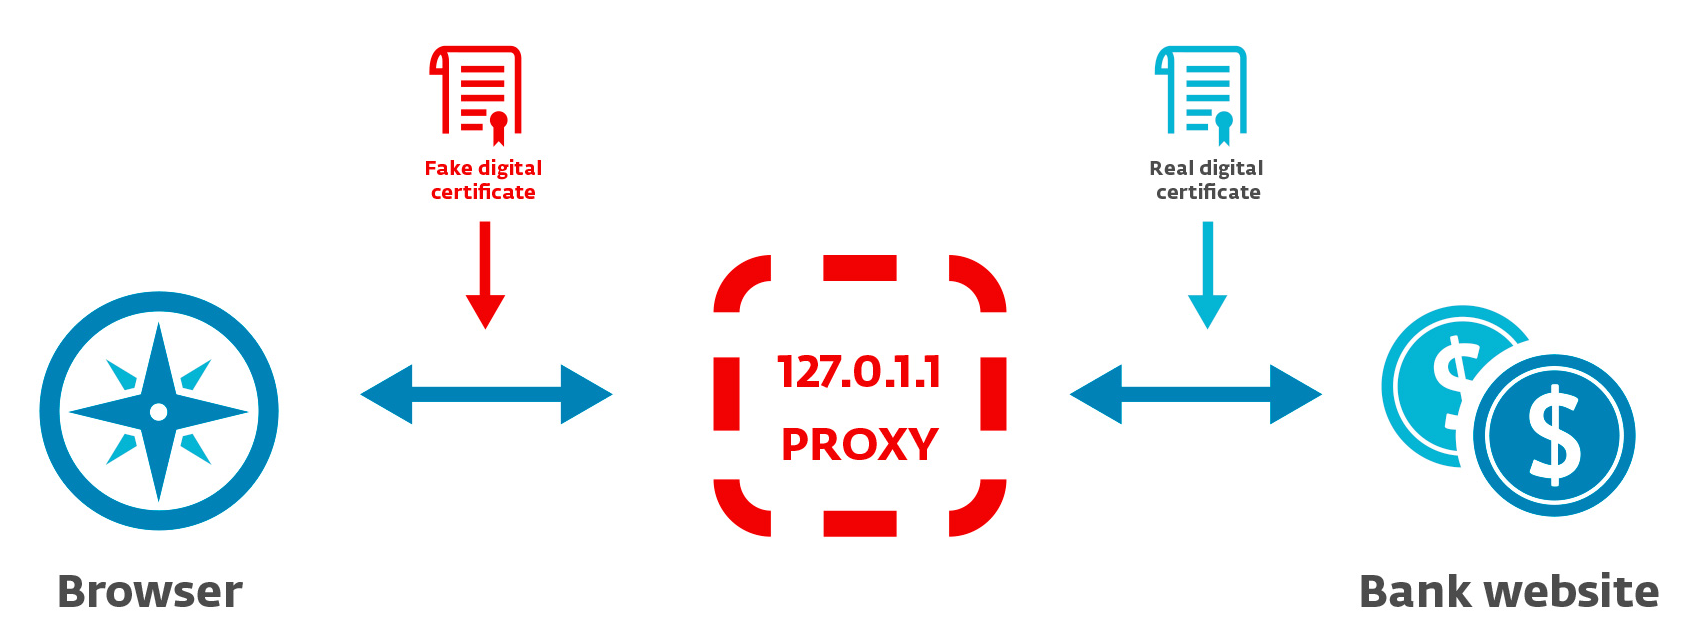
\includegraphics[width=\linewidth]{../medias/interception-https.png}

    \hspace{10cm}

    \begin{columns}
        \begin{column}{0.7\textwidth}
            \begin{block}{Fonctionnement}
                \begin{itemize}
                    \item{Installer un certificat dans le navigateur du client}
                    \item{Faire un proxy https entre client et serveur}
                    \item{Texte en clair entre les deux chiffrements}
                \end{itemize}
            \end{block}

        \end{column}

        \begin{column}{0.3\textwidth}
            \begin{exampleblock}{Scénario}
                \begin{itemize}
                    \item{Entreprise}
                    \item{Antivirus}
                    \item{Attaquant}
                \end{itemize}
            \end{exampleblock}
        \end{column}
    \end{columns}

  \hspace{20cm}

  {\Large \centerline{Pas vraiment une attaque...}}

\end{frame}

\begin{frame}{Attaque HTTPS interception}
    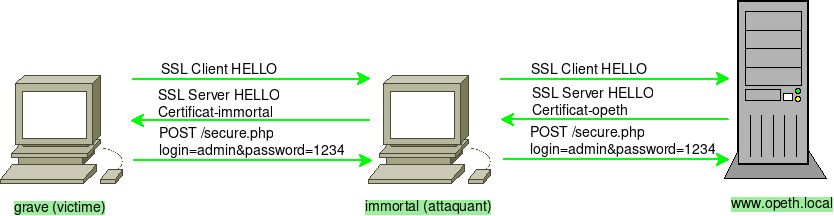
\includegraphics[width=\linewidth]{../medias/https-interception/attack.png}
\end{frame}
